\chapter{Harmonic Motion}
\label{chapter:harmonic-motion}


In Chapter~\ref{chapter:energy}, we studied several oscillatory systems using
the law of conservation of energy, shown in ~\ref{fig:shm-systems}. Using the
energy conservation appoach allows us to solve motion problems quickly, but it
is also clear that the method does not tell us \emph{why} or \emph{how} the
systems oscillate.
\begin{figure}[ht]
  \centering
  \begin{subfigure}{.3\textwidth}
    \centering
    \begin{tikzpicture}[scale=.85]
      \draw[mass] (3,.5) rectangle +(1,1);
      \draw[thick,
        decoration={aspect=.3,segment length=6, amplitude=2.5mm, coil},
        decorate] (0,1)--(3,1);
      \fill[pattern=north east lines] (4.3,0.5)--(4.3,.3)--(-.2,.3)
      --(-.2,2)--(0,2)--(0,.5)--cycle;
      \draw[very thick] (0,2)--(0,.5)--(4.3,.5);
    \end{tikzpicture}
    \caption{Horizontal spring-mass system}
  \end{subfigure}
%    \begin{displaymath}
%      K+U_e=\text{constant}
  %    \end{displaymath}
  \hspace{\stretch1}
  \begin{subfigure}{.3\textwidth}
    \centering
    \begin{tikzpicture}
      \draw[mass] (.7,1.9) rectangle +(.6,.6);
      \draw[thick,
        decoration={aspect=.3,segment length=6, amplitude=2.5mm, coil},
        decorate] (1,5)--(1,2.5); 
      \fill[pattern=north east lines] (0,5) rectangle (2,5.2);
      \draw[very thick] (0,5)--(2,5);
    \end{tikzpicture}
    \caption{Vertical spring-mass system}
%    \begin{displaymath}
%      K+U_e+U_g=\text{constant}
%    \end{displaymath}
  \end{subfigure}
  \hspace{\stretch1}
  \begin{subfigure}{.3\textwidth}
    \centering
    \begin{tikzpicture}
      \fill[pattern=north east lines] (-1,0) rectangle (1,.2);
      \draw[very thick] (-1,0)--(1,0);
      \begin{scope}[rotate=15]
        \draw[thick] (0,0)--(0,-3);% node[midway,right]{$\ell$};
        \shade[ball color=blue] (0,-3) circle (.2);
      \end{scope}
      \draw[dashed,thin] (0,0)--(0,-3);
    \end{tikzpicture}
   \caption{Simple pendulum system}
%    \begin{displaymath}
%      K+U_g=\text{constant}
%    \end{displaymath}
  \end{subfigure}
  \caption{Common examples of harmonic oscillators}
  \label{fig:shm-systems}
\end{figure}
Instead, we must go back to the dynamics (i.e.\ using free-body diagrams and
second law of motion) of such a system, and then solving for the kinematic
properties: position $x$, velocity $v$ and acceleration $a$. Such a system is
called a \textbf{harmonic oscillator}, and the resulting oscillatory motion is
called a \textbf{harmonic motion}.


%In Chapter~\ref{chapter:dynamics}, we showed that Hooke's law for ideal springs
%relates the spring force $\bm F_s$ exerted by a compressed or stretched spring
%onto another object to the spring constant (the stiffness of the spring),
%%$k$\footnote{It is the stiffness of the spring, also called \textbf{Hooke's
%%  constant}, \textbf{force constant}, or the \textbf{spring rate} of the
%%spring. It depends on both the geometry of the spring, as well as the material
%%properties of the spring.},
%and the spring's displacement $\bm x$:
%\begin{equation*}
%  \bm F_s=-k\bm x
%\end{equation*}
%In Chapter~\ref{chapter:energy}, was showed when the spring is compressed or
%stretched, the work done by the spring force is equal to the change in the
%elastic potential energy stored in the spring:
%\begin{equation*}
%  W_s=\int^{x_1}_{x_0}F_s\dl x %=\int^{x_1}_{x_0}(-kx)\dl x
%  =-\frac12kx^2\Big|^{x_1}_{x_0}=-\Delta U_s
%  \quad\text{where}\quad
%  U_s=\frac12kx^2
%\end{equation*}
%Because the work done is equal to the negative change in the potential
%energy:
%\begin{equation*}
%  W_s=-\Delta U_s
%\end{equation*}
%the spring force is a conservative force. In spring-mass systems studied in
%Chapter~\ref{chapter:energy}, the total mechanical energy is always conserved
%when there is no friction, drag, or damping forces. However, applying the law of
%conservation of energy does not immediately show us the type of motion in
%spring-mass systems.



\section{Horizontal Spring-Mass System}

We begin by considering the forces acting on a mass connected horizontally to a
spring without friction, drag, and other damping forces, as shown in
Fig.~\ref{fig:horizontal-spring-mass1}. Three forces act on the mass:
gravitational force $\bm F_g=m\bm g$, normal force $\bm F_n$ at the bottom
surface, and spring force $\bm F_s$ from the stretched/compressed spring.
\begin{figure}[hbt]
  \centering
  \begin{tikzpicture}
    \draw[mass] (5,.5) rectangle (6,1.5);
    \draw[thick,decorate,
      decoration={aspect=.4,segment length=8,amplitude=8,coil}] (0,1)--(5,1);
    \fill[pattern=north east lines] (6.5,.5)--(6.5,.3)--(-0.2,.3)
    --(-.2,2)--(0,2)--(0,.5)--cycle;
    \draw[thick] (6.5,.5)--(0,.5)--(0,2);
    \draw[axes] (6.5,1)--+(.8,0) node[right]{$+$};
    \draw[dashed] (3.5,-.5)--+(0,3) node[above]{Unstretched/Equilibrium};
    \draw[vector] (3.5,0)--(5,0) node[midway,below]{$x$};
    \fill[red] (5.5,1) circle (.08);
    \draw[vector,red] (5.5,1)--(5.5,0) node[below]{$\bm F_g$};
    \draw[vector,red] (5.5,1)--(5.5,2) node[above]{$\bm F_n$};
    \draw[vector,red] (5.5,1)--(4.5,1) node[above]{$\bm F_s$};
  \end{tikzpicture}
  \caption{A horizontal spring-mass system with no friction, drag and damping
    forces}
  \label{fig:horizontal-spring-mass1}
\end{figure}

Since there is no vertical motion, $\sum\bm F_\text{vertical}=0$, $\bm F_g$ and
$\bm F_n$ cancel out. The net force is due only to spring force
$\bm F_e=-k\bm x$ in the horizontal direction. This is true when the spring is
in compression, as well as in extension. (It should be obvious that the
spring in Fig.~\ref{fig:horizontal-spring-mass1} is in extension.) The spring
force is called a \emph{restoring force} because $\bm F_e$ always points
towards the equilibrium position.

Applying second law of motion ($\bm F_\text{net}=m\bm a$) in the horizontal
direction, we can equate the spring force to the mass's horizontal acceleration
($a=\diff[2] xt$):
\begin{important-equation}
  -kx =m\diff[2]xt
  %\underbrace{-kx}_{=F_\text{net}=F_s} =m\diff[2]xt
  \label{eq:ode1}
\end{important-equation}
Eq.~\ref{eq:ode1} is a
\emph{second-order ordinary differential equation with constant
coefficients}\footnote{In many math textbooks, Eq.~\ref{eq:ode1} would be
written in standard form:
\begin{equation*}
  \diff[2]xt + \frac kmx=0
\end{equation*}
} which is a standard problem in calculus. If you are inexperienced in this
type of question, we are looking for a function $x(t)$. When we compare the
left- and right-hand side of Eq.~\ref{eq:ode1}, we would concclude that $x(t)$
must be a function with a second time derivative $\diff[2]xt$ that looks like
$x$, but with a negative sign. The only two functions that can satisfy this
requirement are the sinusoidal functions: $\sin(t)$ and $\cos(t)$, which means
that the motion along the horizontal direction \emph{must} be periodic. We
start with the general form:
\begin{important-equation}
  x(t)=A\cos(\omega t+\theta_0)
  \label{eq:gen-form}
\end{important-equation}
where $A$ is the amplitude of the oscillation, $\omega$ is the angular
frequency of the motion, called \textbf{natural frequency}, and $\theta_0$ is a
phase constant based on initial condition. We will use the cosine function here
for simplicity. Motion in the form of Eq.~\ref{eq:gen-form} is called the
\textbf{simple harmonic motion}\footnote{This type of periodic motion is also
known as \textbf{oscillatory motion}, \textbf{oscillations},
\textbf{vibrations}.}, and such a system is called a
\textbf{simple harmonic oscillator}.
\newpage

\begin{remark}
  In calculus classes, you should be taught that the solution to any ordinary
  differential equation is the linear combination of \emph{all} possible
  solutions. Since both sine and cosine functions are possible solutions to
  Eq.~\ref{eq:ode1}, our solution must be in the form
  \begin{equation*}
    x(t)=c_1\cos(\omega t)+c_2\sin(\omega t)
  \end{equation*}
  where $c_1$ and $c_2$ are coefficients based on initial conditions $x(0)$
  and $v(0)$. Trigonometric identities can be used to show that
  Eq.~\ref{eq:gen-form} is identical to the form of solution above:
  \begin{align*}
    x(t)&=A\cos(\omega t+\theta_0)\\
    &=A\left[\cos(\omega t)\cos(\theta_0)+\sin(\omega t)\sin(\theta_0)\right]\\
    &=\underbracket[1pt]{A\cos(\theta_0)}_{c_1}\cos(\omega t)
    +\underbracket[1pt]{A\sin(\theta_0)}_{c_2}\sin(\omega t)
  \end{align*}
  From an even broader discussions on mathematics, which is not part of the
  discussion here,
  %the solution to any differential equati is a \emph{linear combination} of
  %all the possible solutions.
  all the possible solutions are, in fact, functions that are \emph{orthogonal}
  to each other. Two functions $f(x)$ and $g(x)$ are orthogonal when
  \begin{equation*}
    \int_{-\infty}^\infty f(x)g(x)\dl x=0 
  \end{equation*}
  Much like the basis vectors defining a vector space (for example $\iii$,
  $\jjj$ and $\kkk$ directions representing the $x$, $y$ and $z$ axes) are
  orthogonal, and any vector can be represented as a linear combination of the
  basis vectors, the orthogonal functions are treated as basis vectors
  %(much like the $x$ axis is orthogonal to the $y$ axis)
  and the solution is a vector in this \emph{functional} space.
\end{remark}



Taking the time derivative of Eq.~\ref{eq:gen-form} give us the velocity of
the mass:
\begin{important-equation}
  v(t)=\diff xt=-A\omega\sin(\omega t+\theta_0)
\end{important-equation}
And the second derivative gives us acceleration:
\begin{important-equation}
  a(t)=\diff[2] xt=-A\omega^2\cos(\omega t+\theta_0)=-\omega^2x
\end{important-equation}
We note that the expression of acceleration is related to position $x(t)$ by
the constant $-\omega^2$. Substituting expressions of $x(t)$ and $a(t)$ back
into Eq.~\ref{eq:ode1}, we find that the ODE is satisfied if the natural
frequency $\omega$ is related to the spring constant and mass by:
\begin{important-equation}
  \omega=\sqrt{\frac km}
\end{important-equation}



\textbf{When should we use cosine, and when should be use sine?} Both functions
can be solutions to Eq.~\ref{eq:ode1}, so choosing the ``best'' function is
down to the initial condition (i.e.\ when motion begins at $t=0$). In general,
we prefer a function such that we don't need a phase constant, i.e.\
$\theta_0=0$. If oscillation begins at amplitude $x=A$, shown in
Fig.~\ref{fig:start-from-A}, the $\cos$ function is preferred. If the spring is
initially compressed to $x=-A$, we can use the $-\cos$ function instead.
\begin{figure}[ht]
  \centering
  \begin{subfigure}{.45\textwidth}
    \centering
    \begin{tikzpicture}[scale=.9]
      \draw[mass] (4,.5) rectangle +(1,1);
      \draw[thick,
        decoration={aspect=.3,segment length=2mm, amplitude=2.5mm, coil},
        decorate] (0,1)--(4,1);
      \fill[pattern=north east lines] (5.5,.5)--(5.5,.3)--(-.2,.3)
      --(-0.2,1.5)--(0,1.5)--(0,.5)--cycle;
      \draw[very thick] (0,1.5)--(0,.5)--(5.5,.5);
      \draw[vectors] (2.5,1.65)--(4,1.65) node[midway,above]{$x=+A$};
      \draw[dashed,thick] (2.5,.2)--(2.5,2) node[above=0]{equilibrium};
    \end{tikzpicture}
    \caption{Motion starting at amplitude}
    \label{fig:start-from-A}
  \end{subfigure}
  \begin{subfigure}{.45\textwidth}
    \centering
    \begin{tikzpicture}[scale=.95]
      \draw[mass] (2.5,.5) rectangle +(1,1);
      \draw[thick,
        decoration={aspect=.3,segment length=1.3mm, amplitude=2.5mm, coil},
        decorate] (0,1)--(2.5,1);
      \fill[pattern=north east lines] (5.5,.5)--(5.5,.3)--(-.2,.3)
      --(-0.2,1.5)--(0,1.5)--(0,.5)--cycle;
      \draw[very thick] (0,1.5)--(0,.5)--(5.5,.5);
      \draw[vectors] (3,1)--+(1,0) node[right]{$v=v_\text{max}$};
      \draw[dashed,thick] (2.5,.2)--+(0,1.8) node[above=0]{equilibrium};
    \end{tikzpicture}
    \caption{Motion starting at equilibrium}
    \label{fig:start-from-0}
  \end{subfigure}
\end{figure}  
Conversely, if the mass is given a ``tap'' in the ($+$) direction at $t=0$ to
give it an initial velocity of $v=v_\text{max}$, then the sine function is
preferred, as shown in Fig.~\ref{fig:start-from-0}. In this case, the
oscillator has an initial position of $x(0)=0$. For sine function, we would use
the following functions of time for the mass's position, velocity and
acceleration:
\begin{align*}
  x(t)&=A\sin(\omega t)\\
  v(t)&=A\omega\cos(\omega t)\\
  a(t)&=-A\omega^2\sin(\omega t)
\end{align*}
Mathematically, the two functions only differ by a phase constant of
$\frac{\pi}2$.
%\end{remark}

%The angular frequency for the simple harmonic oscillator is called the
%\textbf{natural frequency}.
The frequency ($f$), i.e.\ the number of oscillations per second, measured in
\emph{hertz} (\si\hertz) of a simple harmonic oscillator is related to the
angular frequency $\omega$ by:
\begin{important-equation}
  f=\frac\omega{2\pi}=\frac1{2\pi}\sqrt{\frac km}
\end{important-equation}
Depending on context or application, the term ``natural frequency'' may refer
to either $\omega$ or $f$.

The period ($T$, measured in seconds) is the reciprocal of the frequency, given
by:
\begin{important-equation}
  T=\frac1f=2\pi\sqrt{\frac mk}
\end{important-equation}
It should be clear that angular frequency ($\omega$), frequency ($f$), and
period ($T$) are all independent of amplitude $A$.


%\begin{frame}{Displacement, Velocity and Acceleration}
%    \begin{align*}
%      x(t)&=A\cos(\omega_0 t-\theta_0)\\
%      v(t)&=-A\omega_0\sin(\omega_0 t-\theta_0)\\
%      a(t)&=-A\omega_0^2\cos(\omega_0 t-\theta_0)=-\omega_0^2x
%    \end{align*}
\begin{figure}[ht]
  \centering
  \begin{tikzpicture}[yscale=.5]
    \draw[axes] (0,-2)--(0,2) node[left]{$x$};
    \draw[axes] (-1,0)--(8,0) node[right]{$t$};
    \draw[very thick,smooth,samples=80,domain=0:7.5]
    plot(\x,{1.5*cos(90*\x)});
      
    \draw[axes] (0,-7)--(0,-3)  node[left]{$v$};
    \draw[axes] (-1,-5)--(8,-5) node[right]{$t$};
    \draw[very thick,smooth,samples=80,domain=0:7.5]
    plot(\x,{-1.5*sin(90*\x)-5});
      
    \draw[axes] (0,-12)--(0,-8)  node[left]{$a$};
    \draw[axes] (-1,-10)--(8,-10) node[right]{$t$};
    \draw[very thick,smooth,samples=80,domain=0:7.5]
    plot(\x,{-1.5*cos(90*\x)-10});
  \end{tikzpicture}
\end{figure}

\begin{remark}
  \textbf{Is $\omega$ the same angular velocity term from circular motion?}
  Yes, it most certainly is. Consider an object moving in uniform circular
  motion about the origin of the $xy$ plane with angular velocity $\omega$.
  In such a case, the angular position of the object would be described by
  \begin{equation*}
    \theta(t)=\omega t+\theta_0
  \end{equation*}
  where $\theta_0$ is the initial angular position of the object. The $x$ and
  $y$ coordinates of this motion are, respectively,
  \begin{align*}
    x(t) &=r\cos(\theta)=r\cos(\omega t+\theta_0)\\
    y(t) &=r\sin(\theta)=r\sin(\omega t+\theta_0)
  \end{align*}
  Both of $x(t)$ and $y(t)$ are in the same form as Eq.~\ref{eq:ode1}. In
  essence, the simple harmonic motion is the projection of a uniform circular
  motion onto an axis. The ``radius'' of the circular motion is the amplitude
  $A$ of the simple harmonic motion. 
  \begin{center}
    \begin{tikzpicture}[scale=.7]
      \draw[axes] (-3,0)--(3,0) node[right]{$x$};
      \draw[axes] (0,-3)--(0,3) node[above]{$y$};
      \draw[dotted] circle (2.5);
      \begin{scope}[rotate=38]
        \draw[vector] (0,0)--(2.45,0) node[midway,above]{$r$};
        \draw[mass] (2.5,0) circle (.1);
        \draw[vector] (2.7,0) arc (0:20:2.7) node[pos=1.15]{$\omega$};
      \end{scope}
      \draw[axes] (1.5,0) arc (0:38:1.5) node[pos=.55,right]{$\theta(t)$};
      \draw[vector] (0,0)--({2.5*cos(38)},0) node[midway,below]{$x(t)$};
      \draw[dashed] ({2.5*cos(38)},0)--({2.5*cos(38)},{2.5*sin(38)});
    \end{tikzpicture}
  \end{center}   
\end{remark}


\begin{remark}
  Another function that we can try as a solution to Eq.~\ref{eq:ode1} is the
  exponential function $x=e^t$, where its derivatives are related to the
  function itself. Again, we start with a general form and take the first two
  time derivatives:
  \begin{equation*}
    x(t)=Ae^{\omega t}\quad\longrightarrow\quad
    \diff xt=A\omega e^{\omega t}\quad\longrightarrow\quad
    \diff[2] xt=A\omega^2 e^{\omega t}=\omega^2x
  \end{equation*}
  It is clear that the problem with using this function is that second
  derivative is missing the negative sign. However, if the exponential function
  is \emph{complex}, i.e.:
  \begin{equation*}
    x(t)=Ae^{i\omega t}
  \end{equation*}
  Then the second derivative \emph{does} in fact have the negative sign:
  \begin{equation*}
    \diff xt=iA\omega e^{i\omega t}\quad\longrightarrow\quad
    \diff[2] xt=i^2A\omega^2 e^{i\omega t}=-\omega^2 e^{i\omega t}=-\omega^2x
  \end{equation*}
  This should not come as a surprise, since the complex exponential function
  and the sinusoidal functions are related:
  \begin{equation*}
    Ae^{i\omega t}=A\left[\cos(\omega t)+i\sin(\omega t)\right]
  \end{equation*}
\end{remark}




\subsection{Energies in the Oscillator}

As the mass oscillates, the kinetic energy of the mass is
\begin{equation}
  K=\frac12mv^2=\frac12m\left[-A\omega\sin(\omega t)\right]^2
\end{equation}
Multiplying out the terms and substutiting for $\omega^2=\frac km$, we have:
\begin{important-equation}
  K=\frac12kA^2\sin^2(\omega t)
\end{important-equation}
Similarly, we can calculate the elastic potential energy stored in the spring
during the oscillation:
\begin{equation}
  U_e=\frac12kx^2=\frac12k\left[A\cos(\omega t)\right]^2
\end{equation}
which gives us:
\begin{important-equation}
  U_e=\frac12kA^2\cos^2(\omega t)
\end{important-equation}
The total energy of the system, which is just the sum of the kinetic and
elastic potential energies, is not suprsingly:
\begin{important-equation}
  E_\text{total}=K+U_e
  =\frac12kA^2\left[\sin^2(\omega t)+\cos^2(\omega t)\right]=\frac12kA^2
\end{important-equation}
We can plot the functions over time:
\begin{figure}[ht]
  \centering
  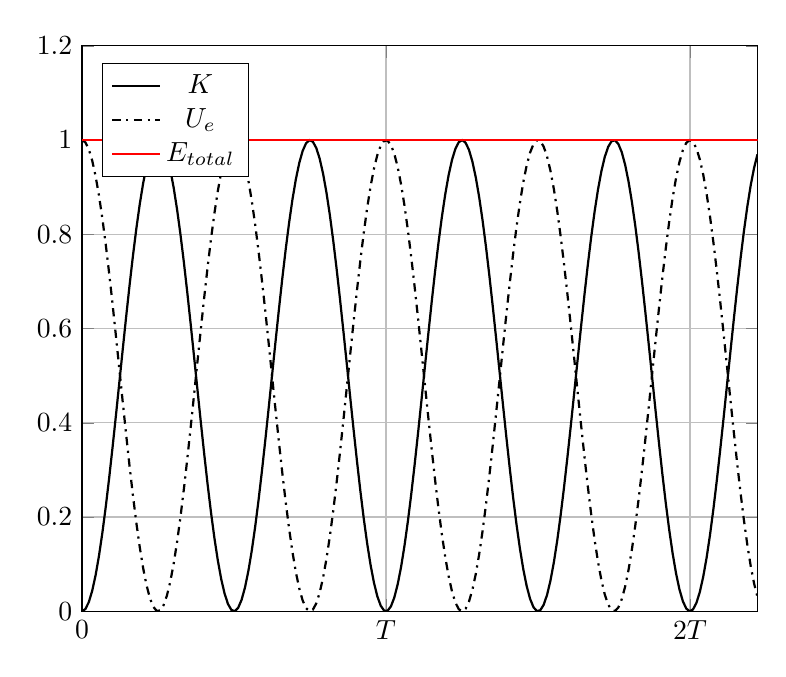
\begin{tikzpicture}
    \begin{axis}[
        width=4in,
        xmin=0,xmax=800,
        ymin=0,ymax=1.2,
        %xlabel=$\theta$ (radian),
        xtick={0,360,720},%,3*pi/8,pi/2},
        xticklabels={0,$T$,$2T$}, %$\dfrac{3\pi}8$,$\dfrac\pi2$
        grid = both,
        legend pos=north west,
      ]
      \addplot[
        thick,
        domain=0:800,
        samples=200,
        style={thick}]{(sin(x))^2};
      \addlegendentry{$K$}
      \addplot[
        thick,dash dot,
        domain=0:800,
        samples=200,
        thick]{(cos(x))^2};
      \addlegendentry{$U_e$}
      \addplot[
        color=red,
        domain=0:800,
        thick]{1};
      \addlegendentry{$E_\text{total}$}
    \end{axis}
  \end{tikzpicture}
\end{figure}
\section{Vertical Spring-Mass System}

For vertical spring-mass systems, shown in
Fig.~\ref{fig:vertical-spring-mass}), we must also consider the gravitational
force $\bm F_g=m\bm g$ which acts along the direction of motion. In this case,
the presence of gravity shifts the equilibrium position to a distance $B$ away
from the unstretched position of the spring.
\begin{figure}[ht]
  \centering
  \begin{tikzpicture}[scale=1.3]
    \draw[mass] (.7,1.7) rectangle (1.3,2.3);
    \draw[thick,
      decoration={aspect=.3,segment length=2mm, amplitude=2.5mm, coil},
      decorate] (1,5)--(1,2.5); 
    \fill[pattern=north east lines] (0,5) rectangle (2,5.2);
    \draw[very thick] (0,5)--(2,5);
    \draw[vector,red] (1,2)--(1,1.2) node[right]{$\bm F_g$};
    \draw[vector,red] (1,2)--(1,2.8) node[right]{$\bm F_s$};
    \fill[red] (1,2) circle (.05);
    \draw[axes] (1,1)--(1,.5) node[below]{$+$};
    \draw[vector] (.3,4)--(.3,2.3) node[midway,left]{$x$};
    \draw[vector] (1.7,4)--(1.7,3.5) node[midway,right]{$B$};
    \begin{scope}[thick,dashed]
      \draw (0,4)--(2,4) node[right]{\scriptsize unstretched};
      \draw (0,3.5)--(2,3.5) node[right]{\scriptsize equilibrium};
    \end{scope}
  \end{tikzpicture}
  \caption{A vertical spring-mass system with no friction and damping force}
  \label{fig:vertical-spring-mass}
\end{figure}
Using the downward direction as the
positive direction of motion, the second law of motion becomes:
\begin{equation}
  mg-kx=m\diff[2]xt
  %\label{eq:ode2}
\end{equation}
Since $F_g$ is constant, the only change is the addition of a constant $B$
in the expression of $x(t)$:
\begin{equation}
  x(t) = A\cos(\omega t+\theta_0) + B\\
  \label{eq:ode1a}
\end{equation}
%  \begin{columns}
%    \column{.3\textwidth}
%    \begin{tikzpicture}[scale=1.3]
%      \draw[mass] (.7,1.7) rectangle (1.3,2.3);
%      \draw[thick,
%        decoration={aspect=0.3,segment length=2mm, amplitude=2.5mm, coil},
%        decorate] (1,5)--(1,2.5); 
%      \fill[pattern=north east lines] (0,5) rectangle (2,5.2);
%      \draw[very thick] (0,5)--(2,5);
%      \draw[vector,red] (1,2)--(1,1.2) node[right]{$\bm F_g$};
%      \draw[vector,red] (1,2)--(1,2.8) node[right]{$\bm F_s$};
%      \fill[red] (1,2) circle (.05);
%      \draw[axes] (1,1)--(1,.5) node[below]{$+$};
%      \draw[vector] (.3,4)--(.3,2.3) node[midway,left]{$x$};
%      \draw[vector] (1.7,4)--(1.7,3.5) node[midway,right]{$B$};
%      \begin{scope}[thick,dashed]
%        \draw (0,4)--(2,4) node[right]{\scriptsize unstretched};
%        \draw (0,3.5)--(2,3.5) node[right]{\scriptsize equilibrium};
%      \end{scope}
%    \end{tikzpicture}

The constant $B$ is the shift of the equilibrium position from the unstretched
position. It is found by equating $F_s=F_g$ and solving for the spring extension
at $x=B$:
\begin{equation}
  B=\frac{mg}k
\end{equation}
%is found by substituting $x$ and $\ddot x$ into the ODE. It is the stretch
%of the spring due to its own weight:
Since $B$ is a constant, velocity and acceleration as functions of time are
unchanged from the horizontal spring-mass case:
\begin{align*}
  v(t) &= -A\omega\sin(\omega t+\theta_0)\\
  a(t) &= -A\omega^2\cos(\omega t+\theta_0)
\end{align*}
Angular frequency (natural frequency) also remains the same as the horizontal
spring-mass system:
\begin{equation*}
  \omega=\sqrt{\frac km}
\end{equation*}

%\subsection{Conservation of Energy in a Spring-Mass System}
%In the spring-mass systems, if there are no frictional losses, then the only
%forces doing work are the spring force (horizontal and vertical) and gravity
%(vertical). Both forces are \emph{conservative}, therefore the total mechanical
%energy is conserved:
%\begin{equation}
%  K + U_s + U_g = K' + U_s' + U_g'
%\end{equation}
%For the horizontal spring-mass system, the total energy of the simple harmonic
%oscillator is:
%\begin{equation}
%  \boxed{E_T=\frac12kA^2}
%\end{equation}

\begin{example}
  A mass suspended from a spring is oscillating up and down. Consider the
  following two statements:
  \begin{enumerate}[nosep]
  \item At some point during the oscillation, the mass has zero velocity but
    it is accelerating
  \item At some point during the oscillation, the mass has zero velocity and
    non-zero acceleration.
  \end{enumerate}
  \begin{enumerate}[nosep]
  \item Both occur at some time during the oscillation
  \item Neither occurs during the oscillation
  \item Only (1) occurs
  \item Only (2) occurs
  \end{enumerate}

  \textbf{Solution:} Will be available when I get around to writing it.
\end{example}

\begin{example}
  An object of mass \SI5{\kilo\gram} hangs from a spring and oscillates with a
  period of \SI{.5}\second. By how much will the equilibrium length of the
  spring be shortened when the object is removed.
  \begin{enumerate}[nosep]
  \item\SI{.75}{\centi\metre}
  \item\SI{1.5}{\centi\metre}
  \item\SI{3.1}{\centi\metre}
  \item\SI{6.2}{\centi\metre}
  \end{enumerate}

  \textbf{Solution:} Will be available when I get around to writing it.
\end{example}



\section{Simple Pendulum}
Aside from spring-mass systems, simple pendulums also exhibit the same kind
of oscillatory motion that we find in spring-mass systems. In the simplest
case, two forces act on the mass: gravitational force $\bm F_g$ and tension
$\bm F_T$, as shown in Fig.~\ref{fig:pendulum1}.
\begin{figure}[ht]
  \centering 
  \begin{tikzpicture}
    \fill[pattern=north east lines] (-1,0) rectangle (1,0.2);
    \draw[thick] (-1,0)--(1,0);
    \begin{scope}[rotate=20]
      \draw[thick] (0,0)--(0,-5) node[midway,right]{$\ell$};
      \shade[ball color=red] (0,-5) circle (.2) node[below right]{$m$};
      \draw[vector,red,dotted] (0,-5)--(-1.5*sin{20},-5)
      node[left,fill=yellow!10]{$mg\sin\theta$};
      \draw[vector,red] (0,-5)--(0,-3) node[left]{$\bm F_T$};
      \draw[vector,red,rotate around={-20:(0,-5)}] (0,-5)--(0,-6.5)
      node[below]{$\bm F_g$};
    \end{scope}
    \draw[axes] (0,-2) arc (270:290:2) node[midway,below]{$\theta$};
    \draw[dashed] (0,0)--(0,-5);
    \draw[dashed] (0,-5) arc (270:295:5);
    \draw[dashed] (0,-5) arc (270:255:5);
  \end{tikzpicture}
  \caption{A simple pendulum deflected by an angle $\theta$}
  \label{fig:pendulum1}
\end{figure}
We have already shown in the discussion for circular motion in
Chapter~\ref{chapter:circ-motion} that when the mass is deflected by an angle
$\theta$, the tangential force is $F_t=-mg\sin\theta$. (The negative sign comes
from the sign convention for circular motion; if $\theta$ is counter clockwise,
in the positive direction, then $F_t$ is clockwise, in the negative direction.)
As we are interested in the pendulum's motion in the angular direction, there
is no need to worry about the radial direction; it does not have to do with the
restoring force.

Substitute $F_t$ into the second law of motion, and cancelling $m$:
\begin{equation}
  F_t=ma_t\quad\rightarrow\quad
  -mg\sin\theta=m\ell\diff[2]{\theta}t
  \quad\rightarrow\quad
  -g\sin\theta=\ell\diff[2]{\theta}t
\end{equation}
Solving this ODE is very difficult because of the $\sin\theta$ term. However,
we can simplify the problem by using the Taylor series expansion of the sine
function:
\begin{equation*}
  \sin\theta
  =\theta-\frac{\theta^3}{3!}+\frac{\theta^5}{5!}-\frac{\theta^7}{7!}+\cdots
\end{equation*}
For small angles of $\theta$, we can use the \emph{small-angle approximation},
where
\begin{equation*}
  \sin\theta\approx\theta
\end{equation*}
and the ODE reduces to the same form as the horizontal spring-mass system that
we have studied in Eq.~\ref{eq:ode1}:
\begin{equation}
  -\frac g\ell\theta = \diff[2]{\theta}t
\end{equation}
For small angles of deflection, the restoring force is approximately
proportional to the angular displacement about the pivot, measured from the
bottom of the swing, just like Hooke's law. Therefore the solution for
$\theta(t)$ is also a sinusoidal function, like the horizontal spring-mass
system:
\begin{important-equation}
  \theta(t)=\theta_\text{max}\cos(\omega t+\varphi)
  \quad\quad\text{simple pendulum, small angles}
\end{important-equation}
where $\theta_\text{max}$ is the maximum deflection of the pendulum (i.e.\ the
amplitude)---which should be kept to a small angle for the solution to be
valid---and $\varphi$ is a phase shift based on the initial condition of the
pendulum.

Again, whether the solution for $\theta(t)$ should be a cosine or a sine
function depends on the initial condition. We want to express the motion
without worrying about the phase constant, as shown in
Fig.~\ref{fig:pendulum-initial}.
\begin{figure}[ht]
  \centering
  \begin{subfigure}{.47\textwidth}
    \centering
    \begin{tikzpicture}
      \fill[pattern=north east lines] (-2,0) rectangle (2,.2);
      \draw[thick] (-2,0)--(2,0);
      \begin{scope}[rotate=25]
        \draw[thick] (0,0)--(0,-3.5);% node[midway,right]{$\ell$};
        \shade[ball color=blue] (0,-3.5) circle (.2)
        node[below right]{$m$} node[above right]{$v(0)=0$};
      \end{scope}
      \draw[axes] (0,-1.5) arc (270:295:1.5)
      node[pos=0,left]{$\theta(0)=\theta_\text{max}$};
      \draw[dashed] (0,0)--(0,-4);
      \draw[dashed] (0,-3.5) arc (270:300:3.5);
      \draw[dashed] (0,-3.5) arc (270:240:3.5);
    \end{tikzpicture}
    \caption{Motion begins at amplitude:
      $\theta(t)=\theta_\text{max}\cos(\omega t)$}
  \end{subfigure}
  \begin{subfigure}{.47\textwidth}
    \centering
    \begin{tikzpicture}
      \fill[pattern=north east lines] (-2,0) rectangle (2,.2);
      \draw[thick] (-2,0)--(2,0);

      \draw[thick] (0,0)--(0,-3.5);% node[midway,right]{$\ell$};
      \shade[ball color=blue] (0,-3.5) circle (.2) node[below right]{$m$};
      \draw[vectors] (0,-3.5)--+(1.3,0) node[right]{$v(0)=v_\text{max}$};

      \draw[dashed] (0,0)--(0,-4) node[pos=.35,left]{$\theta(0)=0$};
      \draw[dashed] (0,-3.5) arc (270:300:3.5);
      \draw[dashed] (0,-3.5) arc (270:240:3.5);
    \end{tikzpicture}
    \caption{Motion begins at $\theta=0$:
      $\theta(t)=\theta_\text{max}\sin(\omega t)$}
  \end{subfigure}
  \caption{Deciding on whether to use sine or cosine functions}
  \label{fig:pendulum-initial}
\end{figure}
The natural frequency of the oscillation $\omega$ is given by:
\begin{important-equation}   
  \omega=\sqrt{\frac g\ell}
\end{important-equation}

\begin{remark}
   \textbf{How small is a ``small angle''?} What constitutes a small angle
  depends on what tolerance (i.e.\ the number of significant figures) is needed
  in the answer. When we plot the difference between $y=\sin\theta$, and our
  approximation $y=\theta$, we can see that both functions agree well near
  $\theta=0$. However, $\sin\theta$ levels off towards $\theta=\frac\pi2$ and
  the linear function (obviously) does not. We can calceulate the percentage
  error:
  \begin{equation*}
    \text{\% Error}=\frac{\theta-\sin\theta}{\sin\theta}\times\SI{100}\percent
  \end{equation*}
  which shown on the right. For a \SI1{\percent} error, the angle of deflection
  should be kept to less than \SI4\degree.
  \begin{center}
    \begin{tikzpicture}
      \begin{axis}[
          width=2.2in,
          xmin=0,xmax=pi/2,
          ymin=0,ymax=pi/2,
          %xlabel=$\theta$ (radian),
          xtick={0,pi/8,pi/4,3*pi/8,pi/2},
          xticklabels={
            0,$\dfrac\pi8$,$\dfrac\pi4$,$\dfrac{3\pi}8$,$\dfrac\pi2$
          },
          grid = both,
          legend pos=north west,
        ]
        \addplot[
          color=blue,
          domain=0:pi/2,
          samples=40,
          style={thick}]{sin(x*180/pi)};
        \addlegendentry{$\sin\theta$}
        \addplot[
          color=red,
          domain=0:pi/2,
          samples=40,
          thick]{x};
        \addlegendentry{$\theta$}
      \end{axis}
    \end{tikzpicture}
    \begin{tikzpicture}
      \begin{axis}[
          width=2.2in,
          ylabel=\% Error,
          xmin=0,xmax=pi/2,
          ymin=0,ymax=60,
          %xlabel=$\theta$ (radian),
          xtick={0,pi/8,pi/4,3*pi/8,pi/2},
          xticklabels={
            0,$\dfrac\pi8$,$\dfrac\pi4$,$\dfrac{3\pi}8$,$\dfrac\pi2$
          },
          ytick={0,10,...,60},
          legend pos=north west,
          grid = both,
        ]
        \addplot[
          color=violet,
          domain=0:pi/2,
          samples=40,
          style=thick
        ]{abs(sin(x*180/pi)-x)/sin(x*180/pi)*100};
      \end{axis}
    \end{tikzpicture}
  \end{center}
\end{remark}



\subsection{Velocity and Acceleration}

We can take the time derivative of $\theta(t)$ to find the angular velocity and
velocity about the pivot of the pendulum:
\begin{important-equation}
  \diff{\theta}t=-\theta_\text{max}\omega\sin(\omega t)
  \quad\to\quad
  v(t)=\ell\diff{\theta}t=-\ell\theta_\text{max}\omega\sin(\omega t)
\end{important-equation}
And the second time derivative gives us the angular acceleration and and
tangential acceleration about the pivot:
\begin{important-equation}
  \diff[2]{\theta}t=-\theta_\text{max}\omega^2\cos(\omega t)
  \quad\to\quad
  a_t(t)=\ell\diff[2]{\theta}t=-\ell\theta_\text{max}\omega^2\cos(\omega t)
\end{important-equation}



\subsection{The meaning of $\omega$}

The meaning of the ``angular frequency'' term $\omega$ for the simple pendulum
is a bit more abstract than in the spring-mass case. Since we are using a
small-angle approximation, we can ``project'' the pendulum's location onto the
$x$-axis, as shown in Fig.~\ref{fig:abstract-omega}.
\begin{figure}[ht]
  \centering
  \begin{tikzpicture}[scale=.9]
    \fill[pattern=north east lines] (-2,0) rectangle (2,.2);
    \draw[thick] (-2,0)--(2,0);
    \begin{scope}[rotate=25]
      \draw[thick] (0,0)--(0,-3.5);
      \shade[ball color=blue] (0,-3.5) circle (.2) node[right=5]{$m$};
    \end{scope}
    
    \begin{scope}[rotate=10]
      \draw[thick,gray] (0,0)--(0,-3.3);
      \shade[ball color=blue,opacity=.3] (0,-3.5) circle (.2);
    \end{scope}
    
    \begin{scope}[rotate=-20]
      \draw[thick,gray] (0,0)--(0,-3.3) node[midway,left,black]{$\ell$};
      \shade[ball color=blue,opacity=.3] (0,-3.5) circle (.2);
    \end{scope}
    
    \draw[axes] (0,-1.5) arc (270:295:1.5) node[right]{$\theta_\text{max}$};
    \draw[dashed] (0,0)--(0,-4);
    \draw[dashed] (0,-3.5) arc (270:300:3.5);
    \draw[dashed] (0,-3.5) arc (270:240:3.5);

    \draw[axes] (-2,-6)--+(4,0) node[right]{$x$};
    \draw[axes] (0,-8)--+(0,4) node[right]{$y$};
    \draw (0,-6) circle (1.48);
    
    \fill (1.48,-6) circle (.08);
    \draw[red,vectors,rotate around={35:(0,-6)}] (1.48,-6) arc (0:70:1.48)
    node[pos=.2,right]{$\omega$};
    
    \draw[dashed] (1.46,-6)--+(0,2.7);
       
    \fill[gray] (.61,-6) circle (.08);
    \fill[gray!70] (.61,-4.66) circle (.08);
    \draw[dashed] (.61,-6)--+(0,2.5);

    \fill[gray] (-1.2,-6) circle (.08);
    \fill[gray!70] (-1.2,-5.13) circle (.08);
    \draw[dashed] (-1.2,-6)--+(0,2.5);
    
    \draw[thick,|<->|] (-1.48,-6.4)--(1.47,-6.4)
    node[midway,below, text width=60]{
      \scriptsize Harmonic motion along the $x$-axis\par};
  \end{tikzpicture}
  \caption{The meaning of the angular freqency term in pendulum motion}
  \label{fig:abstract-omega}
\end{figure}
Since the pendulum deflects through a small angle, we can desribe its motion as:
\begin{align*}
  x(t) &=\ell\sin\left(\theta(t)\right)\approx\ell\theta(t)\\
  &=\ell\theta_\text{max}\cos(\omega_0 t)
\end{align*}
$x(t)$ is the pendulum's \textbf{lateral displacement}, and it is also a simple
harmonic motion. Now we can relate the oscillation on the $x$ axis to a uniform
circular motion on the $xy$-plane. $\omega$ is the angular frequency
of \emph{that} circular motion.   

\begin{example}
  A simple pendulum consists of a mass $m$ attached to a light string of length
  $\ell$. If the system is oscillating through small angles, which of the
  following is true
  \begin{enumerate}[nosep]
  \item The frequency is independent of the acceleration due to gravity, $g$.
  \item The period depends on the amplitude of the oscillation.
  \item The period is independent of the mass $m$.
  \item The period is independent of the length $\ell$.
  \end{enumerate}

  \textbf{Solution:} Will be available when I get around to writing it.
\end{example}

\begin{example}
  A bucket full of water is attached to a rope and allowed to swing back and
  forth as a pendulum from a fixed support. The bucket has a hole in its
  bottom that allows water to leak out. How does the period of motion change of
  the bucket with the loss of water?
  \begin{enumerate}[nosep]
  \item The period does not change.
  \item The period continuously decreases.
  \item The period continuously increases.
  \item The period increases to some maximum and then decreases again.
  \end{enumerate}

  \textbf{Solution:} Will be available when I get around to writing it.
\end{example}

\begin{example}
  A little girl is playing with a toy pendulum while riding in an elevator.
  Being an astute and educated young lass, she notes that the period of the
  pendulum is $T=\SI{.5}\second$. Suddenly the cables supporting the elevator
  break and all  of the brakes and safety features fail simultaneously. The
  elevator plunges into free fall. The young girl is astonished to discover
  that the pendulum has:
  \begin{enumerate}[nosep]
  \item continued oscillating with a period of \SI{.5}\second.
  \item stopped oscillating entirely.
  \item decreased its rate of oscillation to have a longer period.
  \item increased its rate of oscillation to have a lesser period.
  \end{enumerate}

  \textbf{Solution:} Will be available when I get around to writing it.
\end{example}


\begin{remark}
  We have shown that the simple harmonic motion of the spring-mass system
  (without friction or drag or damping forces) as well as the simple-pendulum
  system with small-angle deflection are all periodic. However, it should be
  noted that while all simple harmonic motion are periodic, not all periodic
  motions are harmonic. The ``qualify'' a motion to be a simple harmonic
  motion, there must be a restoring in the form of Hooke's law:
  \begin{equation*}
    F_\text{restoring}=-kx
  \end{equation*}
\end{remark}

\section{Damped Oscillator}

In reality, there are friction, or drag, or other damping forces present in the
spring-mass system, represented schematically by the shock absorber, as shown
in Fig.~\ref{fig:damping1}.
\begin{figure}[ht]
  \centering
  \begin{tikzpicture}
    \draw[gray,mass] (3,.5) rectangle (4,1.5);
    \draw[thick,draw=gray,decorate,
      decoration={aspect=.4,segment length=5,amplitude=8,coil}] (0,1)--(3,1);
    \fill[gray,pattern=north east lines] (-.2,2)--(-.2,.3)--(6.7,.3)--(6.7,2)
    --(6.5,2)--(6.5,.5)--(0,.5)--(0,2)--cycle;
    \draw[gray,thick] (0,2)--(0,.5)--(6.5,.5)--(6.5,2);
    \draw[axes] (7.25,1)--(8,1) node[right]{$x$};
    \fill[blue!20!white] (5,.8) rectangle (6,1.2);
    \draw[very thick] (4,1)--(5,1);
    \draw[very thick] (5,.8)--(5,1.2);
    \draw[very thick] (4.9,1.2)--(6,1.2)--(6,.8)--(4.9,.8);
    \draw[very thick] (6,1)--(6.5,1);
    \begin{scope}[vector,red]
      \draw (3.5,1)--(3.5,0) node[right]{$\bm F_g$};
      \draw (3.5,1)--(3.5,2) node[right]{$\bm F_n$};
      \draw (3.5,1)--(2.5,1) node[above]{$\bm F_s$};
      \draw (3.5,1)--(4.5,1) node[above]{$\bm F_D$};
    \end{scope}
    \fill[red] (3.5,1) circle (.075);
  \end{tikzpicture}
  \caption{A horizontal spring-mass system with a damping force}
  \label{fig:damping1}
\end{figure}

The ``damping force'' is typically related to velocity, but acting the opposite
direction:
\begin{equation}
  F_D=-bv^n
\end{equation}
where $b$ is a positive constant called the \textbf{damping factor}. For
kinetic friction, which acts in opposite direction to motion, but does not
depend on velocty, we can use $n=0$; for a shock absorber, $n=1$, while
aerodynamic drag, $n=2$, as we have seen in Chapter~\ref{chapter:dynamics}.

For the purpose of our analysis, we will use $n=1$ to approximate a mixture of
these effects. Whether this is actually accurate will depends on specific
problems.
%Of course our choice of using $n=1$ will not be entirely correct
%for every problem, but it is \emph{sufficiently} accurate for a wide range of
%situations.}
With the addition of the damping force, the differential equation for the
%\textbf{damped oscillator}
is obtained again by applying second law of motion, but this time with the
additional term from the damping force, highlighted in red:
\begin{align*}
  \sum F = {\color{blue}F_s} + {\color{red}F_D} &= m{\color{orange}a}\\
  -{\color{blue}kx}-{\color{red}b\diff xt} &= m{\color{orange}\diff[2]xt}
\end{align*}
The equation can be arranged into standard form:
\begin{equation}  
  \diff[2]xt+\frac bm\diff xt+\frac kmx=0
  \label{eq:ode2}
\end{equation}
The solution to Eq.~\ref{eq:ode2} is still relatively straightforward, although
not as simple as the simple harmonic oscillator. For small values of $b$, our
solution has both an exponential decay term and a sinusoidal (oscillatory) term:
\begin{important-equation}
  x(t)=
  \underbracket[1pt]{A_0 e^{-\frac b{2m}t}}_\text{amplitude $A(t)$}
  \cos(\omega t+\theta_0)
  \quad\text{(damped oscillator)}
  \label{eq:damped-solution}
\end{important-equation}
where $A_0$ is the initial amplitude. Like the simple harmonic oscillator,
$A_0$, $\theta_0$, and whether to use a sine or cosine function, are based on
initial conditions. The motion of the mass is called a
\textbf{damped harmonic motion}, and such a system is called a
\textbf{damped harmonic oscillator}.

Unlike the simple harmonic oscillator, the motion of the damped oscillator is
\emph{quasi}-periodic because the oscillation pattern is not perfectly
repeated. The natural frequency\footnote{Because the motion is quasi-periodic,
this frequency should be properly called a ``quasi-frequency''.} $\omega'$ for
the damped oscillator is shifted from the undamped case $\omega$ based on the
damping factor $b$:
\begin{important-equation}
  \omega'=\sqrt{\omega^2-\left(\frac b{2m}\right)^2}
  \quad\text{where}\quad
  \omega=\sqrt{\frac km}
  \label{damping1}
\end{important-equation}
Note that $\omega'<\omega$ (natural frequency decreases) because of the
damping factor $b$.

\textbf{Critical damping} occurs when the damped natural frequency $\omega'$ is
zero, which we can calculate by setting $\omega'=0$ in Eq.~\ref{damping1}, and
solving for the resulting damping constant, which is called the \textbf{critical
  damping constant} $b_c$:
\begin{equation*}
  \sqrt{\omega^2-\left(\frac{b_c}{2m}\right)^2}=0
\end{equation*}
Solving for $b_c$, we have:
\begin{important-equation}
  b_c=2m\omega=2\sqrt{km}
\end{important-equation}
At critical damping, the solution to Eq.~\ref{eq:ode2} for the position of the
mass $x(t)$ is
\begin{equation}
  x(t)=(c_1+c_2t)e^{\frac{b_ct}{2m}}
  \label{eq:critically-damped-solution}
\end{equation}
where $c_1$ and $c_2$ are determined by initial conditions. If a mass is
released at amplitude $A_0$ from rest (i.e.\ $x(0)=A_0$, $\dot x(0)=0$), then
Eq.~\ref{eq:critically-damped-solution} becomes:
\begin{equation}
  x(t)=\left[A_0+\frac{A_0}2t\right]e^{\frac{b_ct}{2m}}
  \label{eq:critically-damped-solution}
\end{equation}
\begin{remark}
  The solution in Eq.~\ref{eq:critically-damped-solution} are really two
  linearly independent solutions:
  \begin{align*}
    x_1(t) &= c_1e^{\frac{b_ct}{2m}} \\
    x_2(t) &= c_2te^{\frac{b_ct}{2m}}
  \end{align*}
  We should not be surprised that both solutions are also orthogonal functions.
\end{remark}
A critically damped system returns to its equilibrium position in the shortest
time with \emph{no} oscillation.
\textbf{EXPAND ON THIS SECTION: Critical or near-critical damping is desired
in many engineering designs (e.g.\ shock absorbers on car suspensions).}

When $b>b_c$, the system becomes \textbf{over-damped}. In such a case, the
solution Eq.~\ref{eq:ode2} is the linear combination of two exponential decay
functions:
\begin{equation}
  x(t)=c_1e^{r_1t}+c_2e^{r_2t}
  \quad\text{where}\quad
  r_1=\frac{-b+\sqrt{b^2-4mk}}{2m}\quad
  r_1=\frac{-b-\sqrt{b^2-4mk}}{2m}\quad
  \label{eq:over-damped-solution}
\end{equation}
Once again, the constants $c_1$ and $c_2$ are based on initial position and
velocity of the mass. In an over-damped system, the motion of the mass is
dominiated by the damping force instead of the spring force, and the resulting
motion is a very slow exponential decay without oscillation.

The effects of the damping constant on a harmonic oscillator is illustrated
in the graph shown in Fig.~\ref{fig:damping-effects}.
\begin{figure}[ht]
  \centering
  \begin{tikzpicture}
    \begin{axis}[
        width=4.5in,
        height=3in,
        xmin=0,xmax=1.4,
        xlabel={Time ($t$) [\si\second]},
        %xtick={0,1,2,3}, %xticklabels={0,$\omega$,$2\omega$,$3\omega$},
        ymin=-1.05,
        ymax=1.5,
        ylabel={Relative Amplitude ($\dfrac x{A_0}$)},
        ytick={-1,-.5,0,.5,1},
        grid=both
      ]
      \addplot[
        color=gray,
        samples=200,
        domain=0:2,
        thin]{cos(deg(10*x))}; % have to convert from radian to degree
      \addlegendentry{Undamped ($b=0$)}
      \addplot[
        samples=200,
        domain=0:1.4,
        thick]{exp(-x)*cos(deg(sqrt(99)*x))};
      \addlegendentry{Underdamped ($b=b_c/10$)}
      \addplot[
        samples=200,
        domain=0:1.4,
        thick,dash dot]{exp(-5*x)*cos(deg(sqrt(75)*x))};
      \addlegendentry{Underdamped ($b=b_c/2$)}
      \addplot[
        color=red,
        samples=50,
        domain=0:1.4,
        thick]{(1+2*x)*exp(-10*x)};
      \addlegendentry{Critically damped ($b=b_c$)}
      \addplot[
        color=pink,
        samples=50,
        domain=0:1.4,
        thick]{exp(-4*x)};
      \addlegendentry{Over damped ($b=2b_c$)}
    \end{axis}
    %\node[right,gray] at (5.9,1){\scriptsize Undamped};
    %\node[right] at (1.8,1){\scriptsize$b=\dfrac{b_c}{10}$};
    %\node[right] at (1.5,2.7){\scriptsize$b=\dfrac{b_c}2$};
    %\node[right,red, text width=2cm,align=center] at (.7,4.3){\scriptsize
    %  Critically\\damped};
    %\node[right,pink] at (.8,5.5){\scriptsize Overdamped};
  \end{tikzpicture}
  \caption{Effects of damping constant $b$ on an oscillator}
  \label{fig:damping-effects}
\end{figure}
This example represents
a spring-mass system with a spring constant of $k=\SI{100}{\newton\per\metre}$
and a mass of $m=\SI1{\kilo\gram}$. For simplicity, we use an amplitude of
$A_0=1$. The undamped case (gray line) will have a natural frequency of
$\omega=\sqrt{k/m}=\SI{10}{rad\per\second}$. In a ``light-damped'' system with
a damping factor that is $1/10$ of critical damping, i.e.\ $b=\frac{b_c}{10}$,
the system would clearly oscillate, but each time with decreasing amplitude.
The natural frequencuy $\omega'$ of this damped system is only decreases
slightly, from 10 to $\sqrt{99}=\SI{9.95}{rad\per\second}$, which is only a
\SI{.50}{\percent} decrease. As we increase the damping factor to $1/2$ of
critical, i.e.\ $b=\frac{b_c}2$, the system would only oscillate once before
the oscillation becomes inperceptable. Even now, the damped natural frequency
is still only $\sqrt{75}=\SI{8.66}{rad\per\second}$ which is only a
\SI{13.4}{\percent} decrease. Depending on the tolerance for a design, the
damping for this case would already be considered to be ``near critical''.



\subsection{Energy in a Damped System}
The non-conservative damping force dissipates energy from the oscillator at
a rate of:
\begin{equation}
  P=\diff Et=\bm F_D\cdot\bm v=-bv^2
\end{equation}
As velocity relate to energy by: $(v_{av})^2=E/m$, power dissipation is a
first-order linear ODE:
\begin{equation}
  \diff Et=-\frac bmE
\end{equation}
The solution to the ODE shows the total amount of energy decreases
exponentially with time:
\begin{equation}
  E(t)=E_0e^{-\frac bmt} %=E_0e^{-\frac{t}{\tau}}
\end{equation}




\section{Driven Oscillators}

To keep a damped system going, energy must be added into the system. That means
that positive external work must be done to the system. To ensure that this is
the case, we subject the system to an external forcing function $F_a(t)$ (the
``external applied force'' shown in Fig.~\ref{fig:driven1}) along the direction
of motion that is harmonic with time, with a driving frequency of $\omega_a$:
\begin{equation}
  F_a=F\cos(\omega_at)
\end{equation}
In general, the driving frequency $\omega_a$ is unrelated to the undamped
natural frequency $\omega$ or the damped quasi-frequency $\omega'$, i.e.\
we assume that $\omega_a\neq\omega\neq\omega'$.
\begin{figure}[ht]
  \centering
  \begin{tikzpicture}[scale=1.3]
    \draw[gray,mass] (3,.5) rectangle (4,1.5);
    \draw[thick,gray,decorate,
      decoration={aspect=.4,segment length=6,amplitude=8,coil}] (0,1)--(3,1);
    \fill[gray,pattern=north east lines] (-.2,2)--(-.2,.3)--(6.7,.3)--(6.7,2)
    --(6.5,2)--(6.5,.5)--(0,.5)--(0,2)--cycle;
    \draw[gray,thick] (0,2)--(0,.5)--(6.5,.5)--(6.5,2);
    \draw[fill=blue!10] (4.9,.8) rectangle (5.5,1.2);
    \draw[very thick,gray] (4,1)--(4.9,1);
    \draw[very thick,gray] (4.9,.8)--(4.9,1.2);
    \draw[very thick,gray] (4.8,1.2)--(5.5,1.2)--(5.5,.8)--(4.8,.8);
    \draw[very thick,gray] (5.5,1)--(6.5,1);
    \begin{scope}[vector,red]
      \draw (3.5,1)--(3.5,0) node[right]{$\bm F_g$};
      \draw (3.5,1)--(3.5,2) node[right]{$\bm F_n$};
      \draw (3.5,1)--(2.5,1) node[above]{$\bm F_s$};
      \draw (3.5,.95)--(2,.95) node[below]{$\bm F_a$};
      \draw (3.5,1)--(4.5,1) node[below]{$\bm F_D$};
    \end{scope}
    \fill[red] (3.5,1) circle (.075);
  \end{tikzpicture}
  \caption{A horizontal spring-mass system with a damping force and an external
    applied force.}
  \label{fig:driven1}
\end{figure}
Again, the second-order ordinary differential equation is obtained by
applying the second law of motion:
\begin{equation}
  \sum F=
  \underbracket[1pt]{-kx}_{F_s}\underbracket[1pt]{-bv}_{F_D}+
  \underbracket[1pt]{F\cos(\omega_at)}_{F_a}=ma
\end{equation}
In standard form, the ODE is written as:
\begin{equation}
  m\diff[2]xt + b\diff xt+kx=F\cos(\omega_a t)
  \label{eq:ode3}
\end{equation}
The ODE is similarly to the damped harmonic oscillator: the only difference
between Eq.~\ref{eq:ode2} and Eq.~\ref{eq:ode3} is the additional forcing
function term on the right-hand side. This is a much more difficult problem in
calculus, but nevertheless still a standard problem that is usually taught in a
dedicated differential equation course in university.

The solution to Eq.~\ref{eq:ode3} contains two parts:
\begin{itemize}
\item A \textbf{transient solution} that is obtained by setting $F_a=0$.
  Essentially this is the solution damped harmonic oscillator case, and the
  solution is either an underdamped, critically-damped, or over-damped motion.
  %Eq.~\ref{eq:ode2}, and the solution is already given in
  %Eq.~\ref{eq:damped-solution}.
  The transient solution depends on the initial condition, and regardless of
  the damping factor $b$, the solution will become negligible over time.
\item A \textbf{steady-state solution} which does not depend on the initial
  condition, only on the forcing function $\bm F_a$. Solving for the
  steady-state solution will be left as a difficult calculus exercise.
  This is the solution that we will focus on.
\end{itemize}
The steady-state solution to the driven oscillator is a harmonic motion at the
driving frequency $\omega_a$ of the external force:
\begin{important-equation}
  x(t)=A\cos(\omega_a t+\theta)
  \label{eq:gen-solution3}
\end{important-equation}
%(For those who are interested, Appendix X shows how the steady-state solution
%is derived.)
The amplitude of the oscillation $A$ depends on the natural frequency of the
undamped simple harmonic oscillator $\omega$ (which is a constant), and the
driving frequency $\omega_a$ of the forcing function:
\begin{important-equation}
  A=\frac F{\sqrt{m^2(\omega^2-\omega_a^2)^2+b^2\omega_a^2}}
  \label{eq:amplitude1}
\end{important-equation}
In other words, the amplitude of the driven oscillator is a function of the
driving frequency, i.e.\ $A=A(\omega_a)$.
%And the phase contant is given by:
%\begin{equation}
%  \tan\theta_0=\frac{b\omega_a}{m(\omega^2-\omega_a^2)}
%\end{equation}
Maximum amplitude $A=A_\text{max}$ occurs when $\diff A{\omega'}=0$, which is a
bit difficult and messy to solve. Instead, we can accomplish the same goal by
minimizing the  denominator in Eq.~\ref{eq:amplitude1}, i.e.\ taking the
derivative of the demominator only with respect to external frequency
$\omega_a$, and setting the derivative to 0:
\begin{equation*}
  \diff{}{\omega_a}\left[m^2(\omega^2-\omega_a^2)^2+b^2\omega_a^2\right]=0
\end{equation*}
Taking the derivative and solving for $\omega_a$, we find that maximum
amplitude $A_\text{max}$ occurs when the driving frequency is
\emph{approximately} equal to the natural frequency of the damped system:
%i.e.\ $\omega_a\approx\omega'$.
\begin{important-equation}
  \omega_a=\sqrt{\omega^2-\frac{b^2}{2m^2}}\approx\omega'
\end{important-equation}
Note that the terms inside the square root is \emph{not} the same as in
Eq.~\ref{damping1}!
%In other words, the driving frequency $\omega_a$ at
%maximum amplitude occurs at a frequency that is very close to (albeit slightly
%different from) 

We can plot the amplitude response to different driving frequencies $\omega_a$
(i.e.\ plotting amplitude $A$ as a function of $\omega_a$), as shown in
Fig.~\ref{fig:amp-response}.
\begin{figure}[ht]
  \centering
  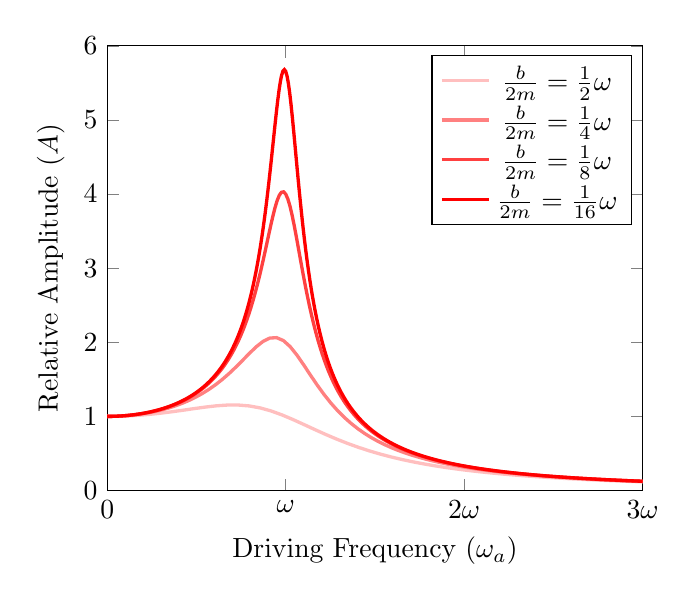
\begin{tikzpicture}
    \begin{axis}[
        width=3.3in,
        xmin=0,xmax=3, xlabel=Driving Frequency ($\omega_a$),
        xtick={0,1,2,3}, xticklabels={0,$\omega$,$2\omega$,$3\omega$},
        ymin=0,ymax=6, ylabel=Relative Amplitude ($A$),
        ytick={0,1,2,3,4,5,6}
      ]
      \addplot[
        color=red!25,
        samples=50,
        domain=0:3,
        very thick]{1/sqrt((1-x^2)^2+x^2)};
      \addlegendentry{$\frac b{2m}=\frac12\omega$}
      \addplot[
        color=red!50,
        samples=80,
        domain=0:3,
        very thick]{1/sqrt((1-x^2)^2+x^2/4)};
      \addlegendentry{$\frac b{2m}=\frac14\omega$}
      \addplot[
        color=red!75,
        samples=250,
        domain=0:3,
        very thick]{1/sqrt((1-x^2)^2+x^2/16)};
      \addlegendentry{$\frac b{2m}=\frac18\omega$}
      \addplot[
        color=red,
        samples=400,
        domain=0:3,
        very thick]{1/sqrt((1-x^2)^2+x^2/32)};
      \addlegendentry{$\frac b{2m}=\frac1{16}\omega$}
    \end{axis}
  \end{tikzpicture}
  \caption{Amplitude response to the driving frequency $\omega_a$.}
  \label{fig:amp-response}
\end{figure}
It shows that, for a lightly-damped system (i.e.\ damping factor $b$ much
smaller than critical), amplitude response is greatest when
$\omega_a\approx\omega'\approx\omega$, and that lower the damping factor $b$,
the higher and narrower the peak is. But as the damping factor increases, and
the damping force begin to dominate, the maximum amplitude will occur at lower
and lower frequencies. Once the driven oscillator has reached its maximum
amplitude for that driving frequency, the power delivered to the system by the
forcing function will be equal to the power dissipated by the damping force(s).

The phase constant $\theta$ in Eq.\ref{eq:gen-solution3} also depends on the
driving frequency $\omega_a$.
\begin{important-equation}
  \tan\theta=\frac{b\omega_a}{m(\omega^2-\omega_a^2)}
  \label{eq:forced-oscillator-phase-shift}
\end{important-equation}
When $\omega_a=\omega$ is substituted into the phase shift expression, the
right-hand side becomes undefined. From this, we obtain a phase shift of
$\theta=\pi/2$. Taking derivative of $x(t)$ for velocity $v(t)$, and
substituting $\theta=\pi/2$:
\begin{equation}
  v(t)=\dot x
  =-A\omega_a\sin(\omega_a t-\frac{\pi}2)
  =A\omega_a\cos(\omega_a t)
\end{equation}
At resonance, the object is always moving in the same direction as the
driving force:
\begin{align*}
  v(t)&=A\omega_a\cos(\omega_a t)\\
  F_a(t)&=F\cos(\omega_a t)
\end{align*}
This also makes sense from a work-energy perspective, because now the
external force is doing positive work to the system.

%\textbf{Resonance} is caused by in-phase excitation near the natural
%frequency. This means that the frequency of the driving force is
%\emph{approximately} equal to the natural frequency of the damped oscillator:
%\begin{equation}
%  \omega_a=\sqrt{\omega^2-\frac{b^2}{2m^2}}
%  \quad\text{where}\quad\omega=\sqrt{\frac km}
%\end{equation}
%For a lightly damped system, $\omega_a\approx\omega\approx\omega$. Also, the
%driving force follows the motion of the oscillator.
%
